\documentclass[sigconf,10pt,nonacm=true]{acmart}
\title{The Impact of Object Immutability on Some Class Cohesion Metrics}

\author{Yegor Bugayenko}
\affiliation{\institution{Huawei Technologies Co., Ltd.}}
\email{yegor.bugayenko@huawei.com}
\author{Sergey Zykov}
\affiliation{\institution{Higher School of Economics}}
\email{szykov@hse.ru}

\usepackage[utf8]{inputenc}
\usepackage{amsmath}
\usepackage{graphicx}
\usepackage{tikz}
\usepackage{pgfplots}
\usepackage{verbatimbox}
\usepackage{interval}
% \usepackage{hyperref}
\usepackage{minted}
  \setminted{fontsize=\footnotesize}
  \setminted{breaklines}
  \usemintedstyle{bw}
\newcommand{\code}[1]{\texttt{#1}}
\newenvironment{nicetable}
  {\setlength{\parindent}{0em}\medskip\small}
  {\medskip}
\begin{document}

\begin{abstract}
Class cohesion is a degree that demonstrates how tightly class
inner elements, like methods and attributes, are bound or related
to one another. Higher cohesion is a trait of good design that
leads to better maintainability.
An immutable object is an object whose state cannot
be modified after it is created.
The goal of this research was to analyze whether immutable objects
are more cohesive and, because of that, more maintainable.
\end{abstract}

\maketitle

%%%%%%%%%%%%%%%%%%%%%%%%%%%%%%%%%%%%%%%%%%%%%%%%%%%%%%%%%%%%%%%%%%%%%%%%%%%%%%%%%%%%%%%%%%%%%%%%%%%%%%%%%%%%%%%%%%%%%%%
%%%%%%%%%%%%%%%%%%%%%%%%%%%%%%%%%%%%%%%%%%%%%%%%%%%%%%%%%%%%%%%%%%%%%%%%%%%%%%%%%%%%%%%%%%%%%%%%%%%%%%%%%%%%%%%%%%%%%%%
%%%%%%%%%%%%%%%%%%%%%%%%%%%%%%%%%%%%%%%%%%%%%%%%%%%%%%%%%%%%%%%%%%%%%%%%%%%%%%%%%%%%%%%%%%%%%%%%%%%%%%%%%%%%%%%%%%%%%%%
\section{Introduction}

Class cohesion, defined by~\citet{yourdon78}
as a degree of how tightly bound or related its internal
elements are to one another,
is considered by~\citet{kabaili01} to be one of the most
important object-oriented software attributes.
A class with low cohesion has disparate and non-related members;
cohesion can be used to identify the poorly designed
classes~\citep{badri08,basili96,chowdhury11}.

An immutable object, as defined by~\citet{goetz05}, is
an object whose state cannot be modified after it is created. Immutable
objects have a number of well-known advantages. First, according to~\citet{bloch06},
they are thread-safe by definition, which means that they can be safely shared between
concurrent threads without any fear of collisions. Second,
according to~\citet{hakonen99}, their usage
is side-effect free, which means that they can be passed to other methods
and functions with full confidence that they will remain intact, no matter
what will happen there. Third, according
to~\citet{nayebi17}, the ``identity mutability'' problem disappears
when objects are immutable, which surfaces when the object's identity is a
derivative of its state. According to~\citet[pp.74--93]{eo1} and~\citet{nayebi17},
there are many other advantages.

This is a perfect example of a mutable Java class:

\begin{minted}{text}
class Book {
  private int id;
  int setId(int i) {
    this.id = i;
  }
}
\end{minted}

An object of this class is capable of modifying its state \code{id} after creation:

\begin{minted}{text}
Book book = new Book();
// Here the state is NULL
book.setId(123);
// Here the state equals to 123
\end{minted}

To the contrary, the following class is immutable since
its state \code{id} can't be modified
after being encapsulated through the constructor, anyhow:

\begin{minted}{text}
class Book {
  private final int id;
  Book(int i) {
    this.id = i;
  }
}
\end{minted}

According to~\citet{li93}, ``it seems logical that the more cohesive a class is,
the easier the class is to maintain.''
Highly cohesive classes, according to the very definition of cohesiveness,
are more maintainable because their design is more focused and easier to understand.
In their research, \citet{dallal13} demonstrated that
``classes with higher cohesion values are more maintainable
than those with lower cohesion values.''
Better maintainability is an obvious objective of any software development.
Thus, high cohesiveness is what classes in object-oriented programming must aim for.

The question is whether making classes immutable helps them become more
cohesive. An empirical analysis of a large group of classes from open
source Java artifacts was performed to find an answer to this question.

%%%%%%%%%%%%%%%%%%%%%%%%%%%%%%%%%%%%%%%%%%%%%%%%%%%%%%%%%%%%%%%%%%%%%%%%%%%%%%%%%%%%%%%%%%%%%%%%%%%%%%%%%%%%%%%%%%%%%%%
%%%%%%%%%%%%%%%%%%%%%%%%%%%%%%%%%%%%%%%%%%%%%%%%%%%%%%%%%%%%%%%%%%%%%%%%%%%%%%%%%%%%%%%%%%%%%%%%%%%%%%%%%%%%%%%%%%%%%%%
%%%%%%%%%%%%%%%%%%%%%%%%%%%%%%%%%%%%%%%%%%%%%%%%%%%%%%%%%%%%%%%%%%%%%%%%%%%%%%%%%%%%%%%%%%%%%%%%%%%%%%%%%%%%%%%%%%%%%%%
\section{Related Work}

Cohesion itself, as an indicator of object-oriented design, was introduced
by~\citet{yourdon78} in 1978 without specifying the exact algorithm of
calculating the metric. Since then, many different algorithms
have been suggested~\citet{izadkhah17}.
Each of them pays attention to certain
parameter of a class or a combination of them, such as the number of methods,
attributes, method arguments, attributes usage frequencies, and so on.
Some studies on existing object-oriented cohesion metrics
even found inconsistencies among some of them~\citep{salem2011,gupta1997}.

Even though high cohesion is known as a virtue of object-oriented design~\citep{kabaili01},
very little work was done to find out what design principles affect
the cohesion. The study of~\citet{patidar2013} concluded that implementation
inheritance negatively affects class cohesion. The research of~\citet{guyomarc2005}
attempted to identify how the usage of AOP aspects affects cohesion.
Recently published research by~\citet{yb-ctors} discovered the relationship
between cohesion and object constructors and suggested that their presence
in cohesion calculating formulas makes a significant impact on the metric.
The research of~\citet{yb-size} demonstrated the relevance betwee class size
and immutability.

So far, to our knowledge, no research has been attempted
to demonstrate the relationship between object immutability and class cohesion.

%%%%%%%%%%%%%%%%%%%%%%%%%%%%%%%%%%%%%%%%%%%%%%%%%%%%%%%%%%%%%%%%%%%%%%%%%%%%%%%%%%%%%%%%%%%%%%%%%%%%%%%%%%%%%%%%%%%%%%%
%%%%%%%%%%%%%%%%%%%%%%%%%%%%%%%%%%%%%%%%%%%%%%%%%%%%%%%%%%%%%%%%%%%%%%%%%%%%%%%%%%%%%%%%%%%%%%%%%%%%%%%%%%%%%%%%%%%%%%%
%%%%%%%%%%%%%%%%%%%%%%%%%%%%%%%%%%%%%%%%%%%%%%%%%%%%%%%%%%%%%%%%%%%%%%%%%%%%%%%%%%%%%%%%%%%%%%%%%%%%%%%%%%%%%%%%%%%%%%%
\section{Five Cohesion Metrics}

According to a summary published by~\citet{izadkhah17},
there are over thirty different metrics to measure
class cohesion. A few of them were selected
for the experiment:

The Normalized Hamming Distance (\textbf{NHD}) class cohesion metric,
introduced by~\citet{counsell06},
measures the similarity in all methods of a class in terms of
the types of their arguments. Let $l$ be the number of
distinct parameter types, $k$ be the number of methods,
and $c_j$ be the number of methods that have a parameter of type $j$,
then,

\begin{equation}
\mathit{NHD} = 1 - \frac{2}{lk(k-1)} \sum_{j=1}^{l} c_j(k-c_j).
\end{equation}

The Sensitive Class Cohesion Metric (\textbf{SCOM}),
introduced by~\citet{fernandez06}, is a
ratio of the summation of connection intensities $C_{i,j}$ of
all pairs $(i,j)$ of $m$ methods to the total number of pairs of methods.
Connection intensity must be given more weight $\alpha_{i,j}$ when such a
pair involves more attributes:

\begin{equation}
\mathit{SCOM} = \frac{2}{m(m-1)} \sum_{i=1}^{m-1} \sum_{j=i+1}^{m} C_{i,j} \times \alpha_{i,j}
\end{equation}

The Method-Method through Attributes Cohesion (\textbf{MMAC}) metric,
introduced by~\citet{dallal07}, is
the average cohesion of all pairs of methods.
Let $k$ be the number of methods, $l$ be the number of distinct parameter types,
and $x_i$ be the number of methods that use type $i$, then,

\begin{equation}
\mathit{MMAC} = \frac{1}{lk(k-1)} \displaystyle\sum_{i=1}^{l} x_i (x_i - 1).
\end{equation}

The Cohesion Among Methods in Class (\textbf{CAMC}), introduced by~\citet{bansiya99},
measures the extent of intersections of individual method parameter
type lists with the parameter type list of all methods in the class.
Let $l$ be the number of distinct parameter types, $k$ be the number
of methods and $p_i$ be the number of distinct parameter
types used by the method $i$, then,

\begin{equation}
\mathit{CAMC} = \frac{1}{lk} \sum_{i=1}^{k} p_i.
\end{equation}

The Lack of Cohesion of Methods (\textbf{LCOM}) is
a correlation between the methods and the local instance variables of a class
(we use the version suggested by~\citet{henderson96}, also known as LCOM5).
Let $m$ be the number of methods, $a$ be the number of
attributes and $\mu_j$ be the amount of methods, which use attribute $j$, then,

\begin{equation}
\mathit{LCOM} = \frac{1}{1 - m} \left( \dfrac{1}{a} \displaystyle\sum_{j=1}^{a} \mu_j \right) - m.
\end{equation}

For all metrics, except LCOM, greater values mean higher cohesion. The LCOM
metric is reversed and demonstrates smaller values for higher cohesion.
To make the discussion easier, we use the inverted version of this metric,
which is:

\begin{equation}
\mathit{LCOM} = 1 - \mathit{LCOM}.
\end{equation}

The values of all metrics are in the $\interval{0}{1}$ interval.

Even though it would be beneficial for this experiment to use all or most
of the available metrics, this is not technically feasible for a number
of reasons. First, the implementation of each metric takes a certain amount of time to understand
the formula, implement the algorithm in Java, and make sure it works as intended.
Second, some metrics were suggested by their authors without thorough testing
with all possible Java code samples. In other words, they work in theory
but can't be implemented ``as is'' in practice, while adapting their
algorithms to the reality of Java code may break their integrity and compromise the
original idea of their authors. The metrics used in this research are implemented
exactly as they were suggested by their authors, and they work correctly with
all available Java classes.

%%%%%%%%%%%%%%%%%%%%%%%%%%%%%%%%%%%%%%%%%%%%%%%%%%%%%%%%%%%%%%%%%%%%%%%%%%%%%%%%%%%%%%%%%%%%%%%%%%%%%%%%%%%%%%%%%%%%%%%
%%%%%%%%%%%%%%%%%%%%%%%%%%%%%%%%%%%%%%%%%%%%%%%%%%%%%%%%%%%%%%%%%%%%%%%%%%%%%%%%%%%%%%%%%%%%%%%%%%%%%%%%%%%%%%%%%%%%%%%
%%%%%%%%%%%%%%%%%%%%%%%%%%%%%%%%%%%%%%%%%%%%%%%%%%%%%%%%%%%%%%%%%%%%%%%%%%%%%%%%%%%%%%%%%%%%%%%%%%%%%%%%%%%%%%%%%%%%%%%
\section{Research Method and Results}

The most popular place for publishing open-source Java artifacts
is the Maven Central Repository~\citep{miller10}.
There were 35211 artifacts found,%
\footnote{\url{https://github.com/yegor256/scrape-maven-central}}
which released at least one version in 2017.
Even though such a large data set constitutes a perfect analysis corpus,
it was decided to only use a subset of the entire Maven Central.
The main reason behind this decision was the amount of time
and computing resources required for the analysis of a single
Java artifact: 100-500 seconds (more than 100 days for the entire Maven Central).

Artifacts with less than one hundred or more than two thousand
\code{.class} files were filtered out.
926 artifacts remained on the list.
This size-based selection criterion was selected due to the following
assumptions: 1) artifacts with fewer classes may represent
abnormally better design due to the attention their developers
were able to pay to each class, 2) artifacts with a lot
of classes may represent the opposite situation, where developers
didn't have enough time to pay attention to the quality of design.
To exclude these abnormalities, it was decided to exclude too big
and too small artifacts and analyze only mid-sized ones.

Cohesion metrics were implemented in the scope of
an open-source Java command line utility and a web system.
It parses Java bytecode \code{.class} files via Javassist~\citep{chiba98},
analyzes its internals with the help of ASM~\citep{bruneton02},
and then creates an XML representation of the entire artifact,
where each class is presented by an XML element.

Interfaces, annotations, enums, anonymous classes,
and classes generated by AspectJ aspect-oriented
framework were filtered out because none of them represent
actual objects in terms of object-oriented design. They are either
auto-generated or surrogates (like enums).

For example, take a simple Java class:

\begin{minted}{text}
class Book {
  private int id;
  int getId() {
    return this.id;
  }
}
\end{minted}

It would be represented in the output XML file as such:

\begin{minted}{text}
<class id='Book'>
  <attributes>
   <attribute public='false' static='false' type='I'>id</attribute>
  </attributes>
  <methods>
    <method abstract='false' ctor='false' desc='()I' name='getId' public='true' static='false'>
      <return>I</return>
      <args/>
    </method>
  </methods>
</class>
\end{minted}

Next, metric-specific XSL transformations~\citep{kay00} were applied to the XML file
in each artifact to generate measurements for each metric.
For example, MMAC metric produced this XML file in
the \code{org.mockito:mockito-all} artifact:

\begin{minted}{text}
<metric>
  <title>MMAC</title>
  <app>
    <class id='InstantiatorProvider' value='1'/>
    <class id='InstantationException' value='0'/>
    <class id='AnswersValidator' value='0.0583'/>
    <class id='ClassNode' value='0.25'/>
    [... skipped ...]
  </app>
</metric>
\end{minted}

Here, \code{AnswersValidator} and \code{ClassNode} are class names,
while \code{0.0583} and \code{0.25} are their corresponding values of
the MMAC formula.

Next, the minimum and the maximum of all \code{value}s in each XML file were found.
For example, in \code{MMAC.xml}, they were 0 and 1 respectively for the Mockito
artifact mentioned above. Then, all classes that
demonstrated values equal to either the minimum or maximum were filtered out. This was done
to minimize the influence of trivial classes that most of the Java artifacts
contain. For example, most metrics would consider this class to be highly cohesive
or even ``perfect,'' despite its lack of usefulness:

\begin{minted}{text}
class Book {
  // The body of the class is empty,
  // no attributes, no methods.
}
\end{minted}

Since most Java artifacts contain classes of a similar kind, it was considered
reasonable to filter out the highest and lowest values to reduce noise. It was
observed that some libraries have many classes with maximum or minimum metric
values. The investigation of more than a hundred of them showed that
all of them are either 1) empty classes with no methods and no attributes,
or 2) utility classes with a large number of static methods and no attributes.

Then, cohesiveness $C_i$ was calculated for each class $i$ in each
artifact as an average of all five metric values.

Then, the size $S_i$ of each class $i$ was calculated as a summary of the
number of methods in the class and the number of attributes. This is
a very rough and primitive metric, but it was required only to help visualize
the entire set of classes on a graph.

Then, all 49,854 classes found were classified into two groups: mutable and immutable.
A class was considered mutable if it had at least one non-final attribute.
This definition of immutability is very far from being strict, but for
this experiment, it was considered to be sufficient enough.

The visual presentation of 40704 mutable classes is in Figure~\ref{fig:1}.

\begin{figure}[h]
  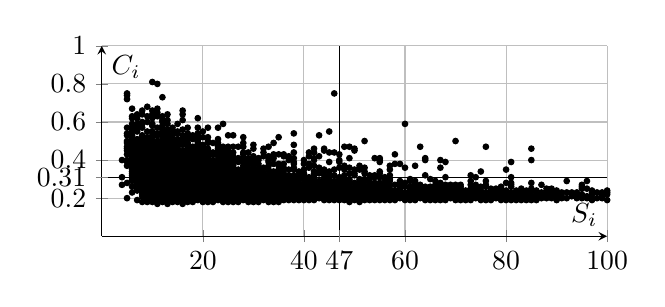
\begin{tikzpicture}\begin{axis}[width=8cm,height=4cm,axis lines=middle, xlabel={$S_i$}, ylabel={$C_i$},xmin=0, xmax=100, ymin=0, ymax=1,extra x ticks={47},extra y ticks={0.3074706211527708},extra tick style={major grid style=black},grid=major]\addplot [only marks, mark size=1pt] table {
15 0.26
16 0.28
18 0.19
28 0.22
16 0.34
29 0.25
57 0.19
16 0.35
25 0.36
17 0.21
35 0.43
9 0.51
16 0.26
8 0.47
21 0.45
19 0.31
12 0.57
37 0.42
29 0.3
63 0.25
72 0.21
110 0.23
15 0.46
37 0.2
46 0.29
6 0.53
18 0.47
65 0.19
20 0.21
9 0.29
19 0.19
32 0.36
85 0.22
35 0.2
58 0.2
45 0.22
40 0.25
69 0.24
17 0.23
10 0.21
10 0.27
21 0.21
22 0.36
12 0.23
34 0.2
26 0.22
18 0.23
14 0.25
16 0.22
10 0.29
22 0.22
11 0.23
13 0.22
23 0.2
51 0.24
27 0.22
10 0.33
28 0.25
63 0.2
26 0.2
20 0.24
20 0.25
24 0.21
54 0.26
24 0.19
20 0.28
7 0.26
25 0.22
38 0.36
47 0.2
60 0.19
111 0.19
22 0.31
33 0.23
77 0.2
22 0.2
13 0.35
76 0.19
55 0.21
43 0.21
86 0.21
20 0.42
20 0.34
12 0.29
18 0.35
32 0.19
14 0.19
11 0.2
57 0.37
24 0.29
10 0.55
9 0.36
10 0.24
29 0.22
58 0.21
70 0.21
24 0.22
19 0.34
38 0.22
13 0.21
10 0.28
19 0.33
28 0.19
17 0.37
14 0.29
31 0.24
61 0.2
14 0.21
16 0.21
39 0.2
41 0.27
38 0.27
9 0.34
44 0.2
7 0.38
15 0.47
30 0.2
8 0.37
15 0.25
13 0.24
12 0.46
67 0.2
56 0.2
33 0.21
32 0.22
163 0.2
15 0.27
37 0.19
28 0.21
21 0.43
12 0.45
16 0.2
11 0.25
33 0.2
25 0.23
17 0.29
45 0.21
68 0.2
37 0.22
72 0.2
19 0.21
33 0.19
39 0.34
21 0.24
8 0.21
20 0.19
50 0.2
9 0.19
21 0.22
10 0.18
11 0.19
36 0.22
37 0.21
54 0.2
13 0.32
11 0.37
24 0.2
29 0.2
26 0.21
12 0.39
27 0.24
24 0.25
17 0.26
10 0.22
28 0.2
7 0.3
46 0.22
43 0.2
23 0.25
38 0.32
40 0.22
26 0.25
50 0.25
54 0.25
89 0.23
28 0.28
33 0.3
32 0.26
28 0.3
56 0.26
55 0.25
66 0.24
30 0.24
44 0.27
42 0.21
39 0.27
34 0.28
32 0.28
70 0.24
53 0.21
44 0.25
63 0.21
34 0.27
34 0.24
37 0.27
45 0.31
41 0.21
34 0.29
48 0.21
65 0.21
45 0.25
36 0.24
56 0.21
62 0.29
50 0.21
49 0.25
47 0.25
43 0.26
53 0.24
72 0.24
61 0.21
67 0.24
45 0.26
41 0.25
56 0.27
71 0.25
38 0.25
82 0.23
71 0.23
51 0.29
55 0.27
49 0.47
57 0.23
82 0.24
83 0.23
47 0.21
18 0.25
18 0.29
10 0.34
26 0.23
87 0.21
84 0.2
22 0.29
13 0.31
8 0.23
33 0.25
20 0.2
32 0.23
8 0.45
20 0.27
24 0.27
52 0.21
22 0.21
35 0.19
17 0.31
23 0.31
30 0.28
15 0.34
8 0.41
19 0.28
15 0.35
8 0.52
10 0.38
43 0.24
35 0.23
60 0.23
28 0.24
10 0.44
25 0.2
7 0.49
18 0.24
12 0.34
16 0.17
54 0.22
8 0.31
9 0.35
29 0.23
23 0.38
17 0.49
55 0.19
16 0.33
13 0.28
15 0.21
26 0.37
88 0.23
21 0.28
9 0.25
15 0.24
17 0.28
18 0.21
27 0.26
27 0.28
10 0.36
14 0.28
16 0.39
17 0.25
56 0.22
12 0.4
11 0.5
33 0.22
11 0.36
22 0.23
48 0.22
24 0.28
18 0.26
14 0.42
20 0.33
15 0.51
21 0.38
15 0.54
29 0.19
15 0.22
7 0.43
12 0.2
10 0.26
11 0.4
12 0.32
14 0.45
23 0.19
83 0.2
11 0.32
21 0.29
40 0.21
19 0.27
50 0.35
13 0.27
16 0.41
32 0.21
51 0.21
37 0.4
38 0.21
10 0.35
24 0.26
40 0.19
52 0.2
26 0.19
14 0.33
26 0.29
74 0.2
27 0.25
17 0.41
18 0.42
24 0.39
34 0.19
21 0.23
71 0.21
7 0.31
31 0.21
19 0.2
22 0.26
25 0.21
46 0.2
58 0.19
55 0.2
19 0.22
31 0.2
46 0.25
64 0.19
13 0.26
31 0.25
52 0.19
19 0.26
79 0.2
70 0.19
79 0.19
43 0.22
88 0.2
82 0.19
64 0.21
97 0.19
40 0.2
73 0.19
17 0.22
49 0.19
64 0.2
112 0.2
121 0.2
85 0.19
139 0.2
112 0.25
88 0.21
9 0.37
18 0.34
10 0.19
6 0.57
8 0.22
9 0.3
21 0.2
16 0.56
12 0.31
8 0.38
16 0.27
13 0.43
27 0.23
16 0.18
15 0.3
21 0.26
9 0.23
15 0.2
118 0.27
5 0.43
17 0.2
25 0.19
6 0.43
13 0.2
29 0.21
59 0.2
71 0.2
153 0.2
42 0.3
38 0.2
42 0.2
11 0.21
18 0.2
45 0.2
154 0.2
66 0.19
75 0.2
17 0.34
11 0.28
32 0.2
104 0.2
36 0.2
50 0.19
11 0.27
14 0.57
13 0.45
30 0.4
17 0.18
20 0.22
23 0.24
44 0.21
15 0.37
30 0.27
22 0.19
32 0.27
16 0.36
12 0.26
23 0.3
27 0.19
12 0.5
79 0.22
31 0.23
25 0.26
33 0.28
82 0.21
29 0.28
59 0.23
54 0.21
22 0.24
23 0.23
27 0.2
41 0.22
26 0.26
68 0.23
27 0.21
62 0.25
35 0.25
11 0.29
14 0.31
26 0.27
21 0.39
14 0.39
23 0.27
34 0.21
64 0.24
42 0.22
30 0.34
49 0.18
20 0.4
17 0.44
14 0.37
49 0.21
18 0.33
60 0.2
17 0.32
26 0.24
19 0.32
97 0.2
36 0.25
22 0.28
25 0.24
26 0.28
18 0.38
35 0.24
19 0.24
78 0.24
16 0.24
22 0.18
16 0.23
6 0.63
13 0.29
15 0.4
25 0.28
37 0.24
70 0.25
13 0.36
13 0.37
21 0.32
14 0.3
20 0.26
13 0.25
18 0.22
9 0.22
20 0.23
7 0.33
12 0.21
11 0.24
23 0.21
24 0.23
11 0.22
20 0.18
41 0.31
35 0.22
8 0.43
31 0.22
51 0.2
35 0.26
27 0.18
102 0.19
7 0.48
17 0.4
713 0.25
12 0.55
9 0.38
23 0.22
11 0.47
11 0.31
8 0.35
52 0.25
57 0.25
9 0.33
24 0.31
39 0.24
35 0.21
42 0.28
15 0.44
18 0.39
21 0.4
22 0.4
19 0.4
9 0.44
19 0.43
22 0.35
20 0.31
10 0.66
21 0.34
22 0.34
19 0.25
71 0.26
137 0.2
10 0.39
19 0.51
28 0.31
99 0.2
11 0.33
39 0.26
26 0.31
31 0.28
34 0.22
10 0.43
15 0.18
75 0.23
59 0.22
52 0.22
54 0.31
16 0.43
41 0.26
129 0.21
141 0.21
137 0.21
238 0.22
250 0.22
254 0.22
355 0.22
361 0.23
365 0.23
505 0.22
36 0.3
37 0.23
52 0.24
7 0.51
14 0.23
34 0.25
21 0.41
21 0.37
7 0.34
25 0.45
30 0.29
21 0.18
44 0.32
99 0.23
91 0.2
10 0.23
16 0.25
44 0.23
27 0.32
7 0.25
42 0.27
87 0.23
106 0.2
9 0.4
67 0.21
14 0.5
5 0.4
15 0.32
23 0.33
65 0.22
77 0.23
34 0.34
48 0.35
32 0.3
30 0.41
42 0.33
15 0.29
19 0.54
34 0.38
33 0.4
12 0.22
8 0.28
7 0.39
38 0.24
94 0.21
33 0.32
19 0.3
9 0.26
8 0.26
31 0.26
10 0.48
15 0.36
22 0.39
57 0.2
23 0.28
25 0.27
11 0.53
16 0.32
27 0.27
29 0.37
24 0.37
29 0.39
40 0.24
45 0.28
23 0.34
17 0.33
28 0.43
15 0.33
65 0.23
11 0.44
12 0.43
9 0.43
38 0.26
11 0.43
14 0.38
38 0.38
25 0.47
18 0.43
12 0.36
20 0.36
35 0.52
18 0.31
101 0.26
25 0.35
77 0.22
10 0.3
20 0.35
9 0.39
8 0.57
22 0.25
78 0.2
53 0.2
14 0.26
13 0.34
15 0.43
6 0.33
5 0.47
14 0.32
15 0.23
8 0.34
33 0.18
12 0.18
12 0.56
7 0.28
135 0.19
59 0.25
24 0.32
11 0.49
11 0.3
7 0.45
11 0.26
9 0.47
17 0.39
36 0.29
17 0.36
16 0.29
48 0.27
9 0.28
8 0.46
16 0.3
24 0.33
84 0.21
14 0.43
30 0.32
41 0.36
5 0.37
6 0.32
22 0.32
17 0.38
6 0.5
8 0.3
15 0.41
21 0.31
41 0.2
10 0.64
10 0.46
16 0.37
17 0.24
30 0.22
83 0.19
6 0.36
11 0.17
11 0.41
16 0.49
28 0.47
51 0.27
53 0.22
9 0.31
19 0.29
27 0.29
41 0.38
67 0.4
7 0.55
25 0.4
19 0.23
22 0.27
16 0.42
25 0.38
26 0.4
24 0.38
12 0.3
11 0.18
12 0.28
38 0.23
86 0.2
23 0.37
20 0.29
12 0.35
47 0.19
140 0.25
76 0.21
134 0.27
109 0.24
6 0.45
26 0.35
74 0.24
76 0.29
100 0.23
109 0.23
96 0.2
34 0.3
12 0.49
85 0.21
43 0.23
15 0.31
19 0.36
14 0.48
67 0.23
27 0.31
35 0.29
51 0.25
70 0.2
79 0.26
53 0.23
41 0.23
81 0.22
44 0.22
25 0.33
18 0.32
47 0.23
52 0.27
34 0.23
48 0.3
76 0.47
66 0.23
12 0.25
7 0.4
39 0.21
32 0.33
5 0.39
38 0.28
73 0.23
13 0.46
206 0.21
23 0.26
46 0.28
30 0.26
55 0.22
72 0.23
18 0.27
6 0.62
14 0.53
11 0.39
32 0.32
111 0.2
21 0.35
21 0.25
17 0.27
31 0.27
30 0.21
14 0.34
12 0.33
23 0.4
18 0.28
51 0.22
41 0.29
35 0.28
36 0.28
49 0.2
13 0.4
6 0.47
37 0.35
47 0.22
14 0.36
33 0.26
93 0.23
45 0.32
59 0.21
66 0.26
65 0.26
79 0.25
46 0.35
59 0.27
63 0.27
49 0.27
64 0.22
69 0.21
47 0.43
49 0.3
69 0.25
30 0.31
14 0.27
58 0.23
24 0.44
23 0.42
74 0.21
25 0.18
33 0.27
90 0.24
79 0.24
77 0.24
54 0.28
60 0.36
60 0.22
46 0.44
109 0.21
89 0.25
118 0.23
105 0.21
101 0.21
101 0.24
136 0.23
183 0.22
206 0.22
45 0.27
44 0.29
52 0.29
74 0.26
43 0.28
64 0.25
55 0.26
53 0.25
48 0.25
49 0.22
67 0.28
90 0.21
74 0.27
88 0.25
145 0.23
68 0.19
10 0.37
8 0.24
14 0.35
48 0.2
50 0.22
68 0.21
143 0.21
62 0.21
93 0.21
159 0.2
14 0.24
67 0.22
28 0.27
15 0.49
17 0.53
28 0.37
7 0.29
8 0.49
7 0.44
24 0.34
11 0.38
13 0.39
13 0.59
12 0.44
9 0.32
14 0.22
14 0.51
18 0.44
13 0.23
16 0.48
197 0.22
13 0.44
21 0.3
18 0.36
150 0.2
43 0.25
56 0.23
17 0.43
27 0.3
17 0.46
72 0.22
24 0.43
71 0.19
182 0.21
76 0.27
73 0.22
21 0.27
18 0.45
188 0.2
54 0.24
6 0.4
125 0.2
95 0.2
20 0.3
81 0.39
62 0.2
64 0.26
117 0.22
16 0.5
26 0.3
37 0.26
66 0.2
56 0.25
87 0.2
15 0.48
20 0.39
12 0.37
50 0.23
13 0.42
73 0.32
1061 0.24
165 0.22
56 0.19
6 0.3
32 0.25
31 0.19
55 0.24
109 0.22
66 0.21
48 0.24
35 0.27
49 0.23
30 0.23
28 0.23
16 0.31
61 0.23
17 0.3
17 0.19
32 0.24
36 0.19
83 0.21
14 0.4
26 0.33
12 0.27
9 0.2
54 0.23
12 0.24
6 0.41
22 0.43
35 0.34
13 0.19
11 0.63
15 0.28
14 0.2
36 0.23
18 0.3
44 0.19
34 0.26
14 0.47
8 0.33
13 0.48
138 0.2
36 0.36
27 0.4
23 0.35
10 0.32
8 0.27
9 0.42
15 0.38
25 0.29
57 0.35
39 0.22
14 0.55
25 0.39
45 0.23
21 0.49
8 0.53
20 0.32
11 0.42
8 0.6
20 0.45
12 0.63
40 0.27
98 0.2
43 0.34
8 0.25
7 0.37
9 0.55
172 0.2
24 0.24
55 0.23
23 0.29
42 0.19
12 0.42
6 0.39
25 0.25
11 0.34
65 0.25
13 0.33
22 0.3
12 0.41
29 0.24
28 0.33
31 0.36
141 0.2
8 0.44
90 0.2
15 0.39
20 0.37
10 0.47
80 0.2
107 0.22
19 0.39
51 0.19
19 0.38
15 0.45
52 0.23
19 0.42
7 0.35
40 0.26
21 0.36
5 0.53
113 0.2
97 0.24
115 0.21
30 0.19
15 0.19
29 0.27
11 0.54
38 0.44
80 0.23
142 0.21
40 0.23
18 0.18
13 0.3
48 0.19
65 0.2
117 0.2
23 0.32
42 0.23
19 0.5
38 0.41
23 0.46
37 0.25
23 0.49
20 0.43
24 0.35
19 0.44
12 0.53
25 0.31
21 0.46
27 0.39
44 0.24
77 0.25
50 0.24
85 0.2
13 0.38
21 0.19
50 0.26
38 0.19
200 0.25
39 0.25
29 0.32
45 0.24
32 0.29
113 0.21
26 0.32
33 0.29
29 0.26
80 0.22
42 0.24
51 0.23
17 0.35
26 0.39
30 0.3
34 0.41
46 0.21
118 0.2
57 0.22
65 0.24
64 0.41
7 0.5
7 0.24
28 0.39
6 0.35
59 0.38
24 0.3
9 0.45
14 0.46
36 0.21
19 0.45
114 0.2
76 0.2
52 0.36
97 0.23
81 0.28
93 0.22
123 0.22
108 0.2
39 0.23
53 0.28
95 0.21
46 0.24
108 0.21
68 0.24
84 0.24
71 0.27
53 0.27
85 0.46
54 0.32
22 0.37
28 0.26
5 0.45
9 0.18
8 0.51
14 0.41
6 0.46
10 0.4
21 0.33
13 0.41
21 0.57
22 0.49
18 0.41
30 0.48
10 0.41
29 0.29
41 0.19
26 0.44
21 0.5
39 0.28
10 0.42
12 0.47
61 0.19
91 0.21
7 0.58
9 0.6
5 0.57
110 0.21
31 0.33
140 0.2
16 0.4
6 0.37
19 0.37
30 0.42
16 0.19
10 0.45
47 0.39
49 0.24
40 0.4
42 0.37
14 0.44
12 0.48
87 0.22
11 0.35
175 0.2
10 0.58
13 0.54
10 0.31
6 0.48
229 0.2
57 0.21
26 0.53
31 0.3
48 0.23
58 0.27
11 0.45
10 0.25
27 0.41
20 0.55
63 0.22
54 0.19
34 0.49
16 0.66
45 0.44
10 0.51
25 0.32
24 0.36
62 0.28
18 0.4
32 0.46
44 0.26
9 0.46
73 0.21
43 0.27
7 0.32
36 0.31
19 0.53
31 0.29
33 0.47
47 0.4
92 0.29
46 0.23
39 0.19
37 0.29
29 0.33
6 0.55
23 0.47
12 0.19
8 0.29
55 0.39
68 0.39
31 0.31
9 0.48
155 0.26
32 0.42
40 0.28
27 0.34
5 0.2
92 0.2
41 0.28
64 0.23
74 0.25
122 0.21
138 0.22
116 0.21
18 0.37
9 0.68
10 0.49
80 0.28
27 0.35
40 0.33
34 0.31
47 0.3
55 0.28
33 0.35
80 0.21
51 0.3
36 0.33
73 0.2
47 0.31
31 0.35
75 0.26
68 0.27
76 0.26
61 0.29
31 0.34
60 0.28
73 0.27
81 0.26
48 0.28
33 0.42
34 0.43
22 0.33
28 0.35
67 0.19
24 0.46
35 0.35
40 0.35
21 0.42
30 0.38
31 0.38
17 0.47
58 0.24
25 0.34
41 0.3
91 0.23
38 0.29
45 0.29
131 0.22
12 0.38
29 0.35
37 0.32
7 0.57
19 0.46
5 0.46
146 0.2
6 0.52
6 0.34
58 0.43
53 0.32
75 0.19
86 0.22
60 0.26
138 0.21
38 0.48
32 0.44
23 0.44
31 0.41
58 0.22
89 0.22
209 0.2
388 0.21
30 0.25
47 0.26
13 0.55
16 0.45
28 0.32
30 0.33
6 0.38
128 0.2
16 0.38
80 0.24
94 0.22
35 0.3
62 0.22
104 0.21
73 0.24
82 0.2
81 0.21
47 0.27
12 0.73
48 0.32
35 0.37
70 0.5
71 0.22
31 0.18
50 0.28
6 0.42
25 0.43
77 0.19
11 0.67
7 0.42
126 0.19
110 0.2
45 0.19
11 0.65
62 0.19
115 0.2
41 0.24
9 0.21
31 0.32
33 0.31
9 0.24
12 0.58
61 0.22
8 0.66
28 0.29
6 0.59
35 0.38
28 0.4
24 0.45
57 0.29
50 0.32
38 0.35
34 0.33
15 0.42
33 0.37
90 0.22
30 0.35
59 0.29
103 0.19
109 0.2
129 0.2
13 0.53
29 0.18
36 0.38
23 0.51
35 0.18
23 0.39
23 0.36
81 0.2
8 0.36
40 0.3
9 0.27
70 0.22
75 0.22
8 0.42
80 0.19
86 0.19
89 0.2
101 0.2
158 0.2
134 0.2
107 0.2
149 0.2
221 0.2
7 0.59
26 0.41
4 0.31
69 0.27
43 0.33
29 0.4
44 0.28
28 0.44
64 0.4
59 0.24
106 0.21
57 0.3
96 0.29
113 0.26
44 0.3
5 0.49
39 0.3
151 0.2
127 0.21
5 0.75
5 0.74
36 0.27
120 0.22
145 0.2
136 0.2
198 0.2
99 0.21
12 0.54
5 0.5
9 0.63
13 0.47
36 0.26
46 0.27
16 0.44
38 0.3
84 0.23
63 0.47
18 0.46
20 0.47
48 0.37
22 0.38
81 0.27
54 0.41
75 0.34
95 0.27
9 0.49
7 0.62
70 0.27
9 0.41
25 0.3
133 0.22
146 0.21
144 0.21
26 0.42
42 0.25
170 0.2
105 0.22
38 0.31
63 0.24
47 0.24
49 0.41
73 0.29
131 0.2
37 0.28
37 0.3
7 0.41
10 0.59
33 0.34
8 0.39
102 0.2
192 0.2
57 0.32
6 0.23
20 0.46
6 0.51
19 0.57
173 0.37
20 0.38
296 0.2
114 0.21
13 0.51
27 0.47
27 0.33
22 0.44
13 0.52
9 0.52
40 0.31
30 0.36
46 0.19
68 0.31
85 0.24
170 0.21
5 0.72
24 0.41
102 0.21
19 0.41
6 0.56
32 0.34
30 0.39
42 0.4
47 0.36
42 0.44
44 0.45
55 0.4
52 0.34
74 0.31
80 0.35
15 0.59
6 0.44
26 0.18
13 0.49
6 0.67
61 0.3
41 0.44
36 0.43
66 0.29
49 0.33
43 0.42
8 0.59
13 0.64
53 0.26
51 0.18
57 0.27
63 0.26
66 0.25
156 0.2
95 0.26
85 0.25
56 0.29
62 0.27
53 0.3
51 0.26
97 0.22
10 0.53
26 0.47
24 0.18
237 0.23
8 0.32
103 0.2
181 0.2
136 0.19
130 0.2
30 0.46
89 0.24
42 0.41
7 0.64
43 0.29
35 0.31
25 0.41
5 0.54
7 0.47
58 0.38
29 0.41
36 0.32
19 0.48
17 0.42
38 0.54
33 0.24
56 0.24
102 0.22
62 0.23
84 0.22
127 0.2
70 0.23
120 0.21
150 0.22
76 0.22
121 0.22
63 0.23
78 0.23
5 0.28
69 0.2
7 0.27
160 0.2
8 0.4
72 0.19
19 0.35
166 0.2
67 0.27
107 0.21
75 0.21
85 0.4
52 0.3
43 0.53
24 0.59
28 0.36
42 0.32
17 0.51
33 0.39
52 0.5
51 0.37
42 0.46
48 0.26
50 0.46
104 0.26
12 0.6
41 0.42
40 0.32
46 0.32
105 0.25
55 0.34
36 0.42
29 0.44
96 0.21
52 0.33
25 0.53
87 0.27
42 0.34
98 0.23
61 0.25
74 0.23
46 0.26
111 0.21
61 0.26
81 0.23
86 0.24
61 0.24
92 0.23
90 0.23
68 0.25
67 0.25
62 0.24
51 0.28
83 0.25
94 0.23
105 0.23
78 0.21
79 0.23
122 0.23
36 0.35
45 0.34
28 0.49
85 0.28
48 0.47
29 0.31
20 0.41
111 0.22
144 0.22
64 0.32
24 0.42
59 0.26
88 0.22
35 0.32
169 0.22
78 0.25
96 0.25
26 0.36
62 0.37
66 0.27
10 0.2
44 0.34
84 0.19
17 0.54
37 0.31
115 0.22
40 0.38
55 0.41
18 0.51
10 0.81
16 0.51
12 0.61
17 0.57
19 0.62
59 0.28
7 0.36
8 0.64
4 0.27
31 0.4
124 0.2
28 0.34
47 0.29
65 0.3
11 0.48
158 0.25
43 0.36
81 0.31
30 0.18
94 0.2
55 0.31
49 0.36
12 0.51
68 0.22
190 0.2
67 0.36
17 0.45
112 0.22
99 0.22
76 0.23
60 0.21
79 0.21
95 0.22
66 0.22
49 0.28
82 0.22
68 0.26
112 0.23
57 0.24
106 0.23
198 0.21
83 0.22
139 0.22
159 0.23
100 0.22
8 0.5
53 0.19
16 0.61
50 0.33
4 0.4
7 0.19
213 0.3
120 0.2
177 0.2
34 0.18
11 0.8
16 0.64
69 0.22
6 0.26
123 0.21
45 0.55
46 0.75
23 0.57
42 0.26
146 0.3
20 0.48
23 0.48
23 0.45
20 0.44
129 0.22
8 0.18
13 0.18
122 0.24
20 0.52
203 0.38
262 0.21
267 0.37
267 0.21
90 0.19
69 0.23
50 0.45
183 0.27
128 0.21
71 0.24
44 0.35
38 0.39
55 0.33
83 0.24
35 0.33
104 0.33
100 0.24
246 0.33
7 0.46
19 0.49
109 0.19
161 0.22
28 0.52
13 0.61
95 0.25
122 0.2
29 0.34
100 0.19
10 0.62
196 0.22
195 0.2
23 0.43
13 0.56
11 0.57
15 0.55
18 0.53
121 0.21
39 0.32
24 0.47
56 0.31
49 0.29
75 0.24
73 0.25
104 0.23
173 0.2
102 0.26
6 0.29
103 0.22
28 0.41
44 0.46
51 0.35
104 0.24
121 0.23
60 0.59
136 0.21
103 0.23
19 0.47
6 0.31
13 0.17
81 0.19
7 0.56
16 0.53
17 0.48
45 0.39
21 0.52
14 0.18
118 0.21
214 0.2
104 0.22
119 0.23
9 0.5
};\end{axis}\end{tikzpicture}

  \caption{Mutable classes}
  \label{fig:1}
\end{figure}

The visual presentation of 9150 immutable classes is in Figure~\ref{fig:2}.

\begin{figure}[h]
  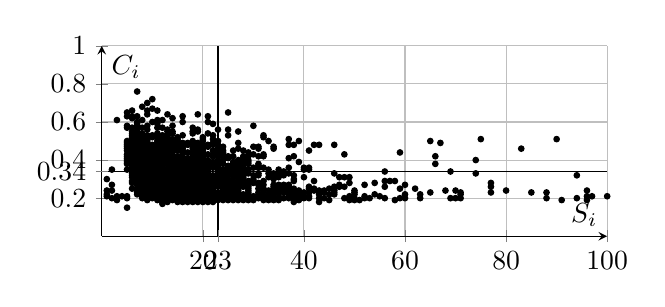
\begin{tikzpicture}\begin{axis}[width=8cm,height=4cm,axis lines=middle, xlabel={$S_i$}, ylabel={$C_i$},xmin=0, xmax=100, ymin=0, ymax=1,extra x ticks={23},extra y ticks={0.34138397502601386},extra tick style={major grid style=black},grid=major]\addplot [only marks, mark size=1pt] table {
15 0.4
7 0.29
11 0.35
13 0.23
62 0.25
7 0.43
5 0.15
19 0.41
14 0.25
22 0.3
39 0.5
11 0.22
38 0.25
11 0.27
9 0.4
6 0.63
16 0.36
5 0.35
7 0.31
20 0.29
9 0.19
14 0.19
37 0.36
22 0.53
15 0.48
9 0.46
7 0.39
13 0.27
14 0.41
5 0.65
5 0.4
74 0.4
22 0.18
33 0.21
25 0.56
14 0.27
8 0.45
23 0.39
24 0.42
22 0.45
9 0.28
12 0.43
13 0.4
7 0.41
21 0.27
16 0.25
9 0.39
9 0.31
14 0.22
7 0.33
9 0.38
15 0.45
16 0.33
13 0.26
20 0.31
18 0.49
9 0.53
8 0.47
17 0.31
11 0.31
7 0.42
9 0.27
7 0.5
12 0.3
23 0.56
27 0.49
13 0.19
6 0.45
18 0.4
11 0.66
25 0.53
15 0.2
9 0.23
30 0.58
9 0.22
5 0.45
10 0.6
11 0.53
16 0.63
12 0.61
23 0.2
7 0.25
46 0.25
10 0.67
23 0.48
14 0.35
13 0.25
8 0.61
8 0.68
32 0.42
37 0.41
7 0.24
7 0.51
7 0.53
11 0.29
12 0.28
32 0.53
25 0.65
8 0.37
8 0.39
16 0.26
12 0.29
14 0.32
20 0.22
9 0.34
2 0.27
5 0.21
3 0.19
24 0.27
5 0.2
4 0.21
12 0.2
17 0.27
32 0.29
29 0.25
9 0.36
6 0.32
13 0.31
24 0.26
12 0.27
22 0.29
11 0.24
13 0.29
29 0.22
10 0.2
7 0.57
32 0.21
19 0.2
15 0.29
9 0.7
14 0.21
20 0.4
5 0.43
6 0.25
7 0.4
10 0.41
15 0.51
10 0.26
29 0.4
29 0.29
13 0.42
28 0.35
26 0.38
6 0.29
46 0.23
24 0.4
27 0.35
37 0.51
11 0.2
48 0.31
8 0.42
10 0.3
10 0.37
6 0.55
11 0.33
27 0.19
51 0.19
20 0.26
9 0.56
9 0.5
6 0.46
18 0.35
21 0.22
14 0.28
28 0.29
9 0.49
13 0.33
8 0.34
46 0.22
11 0.43
7 0.28
8 0.38
10 0.32
29 0.42
31 0.46
11 0.25
49 0.19
14 0.36
14 0.3
43 0.48
8 0.24
19 0.55
14 0.31
17 0.33
6 0.38
5 0.48
5 0.46
5 0.5
5 0.47
13 0.32
6 0.34
26 0.21
16 0.22
12 0.44
22 0.59
14 0.47
9 0.37
10 0.44
15 0.35
13 0.18
20 0.2
18 0.19
8 0.27
37 0.23
15 0.37
24 0.29
24 0.23
22 0.25
31 0.2
19 0.46
21 0.54
9 0.47
9 0.33
9 0.35
9 0.51
16 0.44
25 0.2
13 0.3
8 0.48
32 0.27
12 0.51
35 0.27
20 0.25
6 0.49
6 0.54
9 0.21
9 0.41
15 0.36
43 0.2
69 0.34
65 0.5
12 0.33
10 0.38
41 0.26
15 0.21
22 0.24
17 0.21
31 0.28
75 0.51
19 0.23
19 0.35
23 0.26
26 0.24
65 0.23
13 0.5
44 0.24
43 0.22
38 0.42
50 0.2
18 0.31
16 0.21
14 0.34
12 0.26
8 0.31
16 0.43
21 0.32
37 0.27
20 0.33
17 0.3
13 0.56
16 0.23
16 0.24
13 0.24
11 0.23
7 0.27
8 0.33
15 0.33
22 0.19
55 0.21
26 0.3
70 0.24
88 0.23
131 0.22
16 0.28
28 0.31
25 0.37
21 0.4
8 0.35
31 0.42
26 0.36
9 0.26
12 0.41
16 0.19
9 0.3
11 0.38
18 0.24
12 0.24
9 0.48
21 0.43
17 0.36
41 0.36
21 0.31
33 0.2
33 0.22
13 0.38
13 0.21
12 0.22
36 0.2
20 0.39
15 0.42
9 0.32
5 0.41
22 0.22
10 0.39
14 0.33
18 0.29
13 0.28
11 0.3
21 0.26
17 0.25
34 0.2
25 0.19
6 0.31
10 0.21
38 0.21
24 0.22
24 0.2
26 0.42
39 0.19
41 0.21
10 0.33
27 0.23
9 0.45
7 0.46
19 0.21
14 0.26
22 0.42
26 0.19
10 0.28
40 0.31
35 0.21
35 0.23
34 0.27
33 0.31
34 0.22
38 0.24
15 0.31
18 0.23
8 0.46
11 0.26
6 0.28
24 0.34
10 0.72
13 0.52
13 0.49
13 0.47
16 0.47
16 0.45
16 0.48
14 0.51
15 0.34
9 0.43
15 0.3
11 0.45
28 0.22
34 0.25
23 0.42
17 0.24
59 0.25
77 0.23
7 0.63
12 0.38
12 0.17
10 0.4
11 0.4
14 0.24
59 0.44
5 0.38
11 0.19
28 0.41
26 0.27
13 0.53
26 0.33
13 0.43
8 0.3
36 0.24
15 0.25
18 0.25
10 0.23
12 0.36
8 0.54
30 0.32
49 0.28
14 0.4
19 0.25
19 0.45
9 0.64
23 0.28
27 0.38
7 0.59
12 0.21
29 0.24
32 0.43
13 0.22
16 0.37
8 0.57
11 0.21
15 0.22
30 0.2
13 0.35
10 0.29
12 0.39
19 0.32
8 0.32
7 0.37
17 0.49
45 0.19
14 0.42
6 0.57
11 0.41
31 0.27
29 0.28
8 0.44
14 0.2
85 0.23
23 0.32
18 0.33
43 0.23
50 0.22
14 0.38
25 0.21
13 0.36
7 0.36
6 0.41
21 0.35
35 0.32
29 0.38
27 0.37
44 0.2
32 0.52
74 0.33
67 0.49
8 0.23
6 0.5
8 0.25
41 0.25
35 0.31
16 0.38
19 0.29
19 0.24
10 0.34
16 0.2
37 0.2
63 0.2
96 0.24
57 0.29
56 0.29
139 0.22
8 0.43
18 0.21
13 0.64
19 0.22
35 0.33
10 0.46
22 0.26
90 0.51
71 0.23
31 0.23
28 0.33
28 0.45
31 0.25
94 0.2
11 0.48
42 0.25
39 0.39
60 0.2
69 0.2
13 0.45
10 0.42
9 0.44
19 0.43
8 0.36
18 0.32
68 0.24
8 0.21
15 0.19
11 0.39
6 0.52
17 0.26
10 0.25
18 0.54
11 0.42
12 0.23
16 0.27
8 0.52
17 0.23
7 0.35
9 0.29
7 0.48
14 0.44
20 0.32
34 0.26
20 0.21
2 0.24
19 0.56
25 0.33
8 0.41
13 0.44
27 0.22
20 0.42
18 0.41
17 0.41
7 0.38
29 0.34
20 0.23
7 0.34
40 0.21
28 0.38
37 0.21
37 0.25
26 0.26
18 0.27
53 0.2
21 0.23
41 0.2
49 0.31
25 0.24
39 0.22
63 0.22
46 0.24
34 0.23
18 0.46
7 0.6
28 0.3
15 0.18
29 0.21
10 0.27
6 0.39
14 0.54
23 0.29
15 0.26
15 0.41
12 0.46
31 0.22
70 0.2
32 0.19
15 0.27
12 0.37
71 0.2
11 0.28
14 0.49
17 0.38
11 0.34
20 0.45
21 0.19
20 0.27
11 0.44
26 0.23
12 0.34
14 0.23
10 0.22
21 0.29
6 0.66
20 0.46
23 0.5
17 0.48
27 0.28
26 0.39
40 0.2
24 0.35
23 0.35
15 0.24
31 0.37
46 0.33
13 0.34
12 0.31
16 0.29
28 0.32
14 0.55
12 0.45
9 0.42
21 0.28
18 0.3
6 0.51
16 0.6
18 0.22
14 0.39
20 0.35
10 0.36
21 0.24
18 0.39
41 0.35
40 0.36
27 0.31
40 0.35
26 0.28
15 0.28
26 0.34
19 0.38
22 0.36
7 0.47
28 0.26
6 0.42
11 0.46
11 0.52
23 0.22
7 0.55
12 0.32
15 0.52
16 0.41
20 0.51
21 0.25
33 0.35
29 0.27
29 0.33
25 0.26
28 0.42
27 0.26
21 0.48
27 0.46
29 0.44
24 0.47
10 0.45
21 0.36
10 0.35
19 0.34
12 0.49
38 0.48
46 0.48
26 0.45
30 0.47
34 0.47
42 0.48
24 0.44
16 0.35
13 0.2
12 0.4
39 0.21
48 0.26
97 0.21
100 0.21
71 0.22
96 0.21
45 0.25
107 0.29
121 0.22
130 0.23
130 0.22
134 0.19
11 0.57
26 0.32
32 0.24
14 0.58
9 0.66
13 0.48
26 0.2
39 0.2
20 0.37
26 0.22
28 0.4
11 0.36
10 0.24
12 0.42
6 0.48
16 0.3
25 0.29
20 0.24
23 0.3
15 0.38
18 0.37
21 0.38
30 0.36
30 0.21
22 0.32
21 0.2
50 0.23
22 0.39
28 0.37
26 0.37
29 0.35
11 0.37
31 0.33
34 0.32
17 0.22
16 0.18
27 0.55
27 0.39
80 0.24
27 0.24
17 0.19
20 0.44
22 0.51
23 0.43
30 0.43
21 0.34
38 0.29
22 0.48
24 0.43
33 0.5
7 0.22
22 0.43
31 0.38
35 0.35
30 0.3
66 0.38
83 0.46
94 0.32
38 0.3
91 0.19
136 0.22
35 0.2
29 0.26
24 0.28
2 0.35
2 0.2
1 0.21
22 0.49
11 0.49
9 0.24
25 0.22
3 0.21
24 0.32
21 0.47
5 0.39
30 0.28
11 0.54
17 0.4
17 0.28
19 0.26
30 0.29
14 0.37
10 0.52
23 0.37
17 0.29
28 0.36
18 0.42
20 0.47
7 0.44
23 0.45
18 0.44
46 0.26
11 0.5
24 0.31
1 0.3
22 0.23
27 0.21
23 0.19
7 0.3
6 0.33
3 0.61
16 0.49
22 0.31
47 0.31
21 0.33
19 0.3
19 0.37
7 0.45
15 0.5
34 0.19
33 0.19
20 0.19
18 0.18
17 0.18
27 0.33
28 0.27
10 0.53
8 0.28
21 0.3
14 0.48
39 0.24
25 0.32
8 0.51
1 0.22
1 0.24
18 0.26
34 0.46
22 0.2
28 0.28
29 0.19
56 0.2
58 0.19
6 0.53
54 0.22
35 0.25
44 0.23
30 0.19
10 0.31
7 0.58
205 0.53
6 0.36
8 0.22
28 0.21
6 0.37
19 0.18
15 0.32
59 0.2
21 0.21
28 0.19
7 0.32
12 0.35
38 0.32
48 0.2
25 0.42
13 0.41
36 0.23
10 0.43
31 0.47
16 0.46
8 0.4
19 0.64
19 0.36
14 0.29
8 0.26
16 0.31
17 0.37
23 0.4
21 0.6
54 0.28
15 0.23
60 0.27
52 0.27
23 0.44
40 0.23
34 0.3
19 0.27
22 0.27
35 0.26
37 0.26
37 0.22
107 0.28
21 0.37
9 0.58
77 0.26
60 0.22
12 0.19
19 0.39
13 0.39
36 0.32
33 0.33
8 0.49
11 0.47
45 0.22
49 0.21
27 0.2
19 0.19
50 0.19
11 0.59
12 0.57
6 0.44
12 0.53
11 0.61
16 0.39
20 0.48
31 0.32
25 0.3
20 0.52
7 0.76
50 0.24
9 0.52
58 0.29
7 0.23
9 0.2
27 0.4
19 0.49
66 0.42
20 0.36
19 0.48
56 0.34
33 0.24
12 0.47
17 0.35
18 0.38
20 0.43
20 0.5
25 0.35
47 0.27
20 0.41
24 0.45
20 0.34
24 0.24
31 0.36
24 0.21
23 0.23
41 0.23
5 0.63
32 0.25
5 0.42
16 0.53
22 0.38
23 0.33
23 0.36
37 0.48
48 0.43
17 0.32
20 0.18
10 0.48
6 0.62
5 0.49
26 0.35
19 0.31
13 0.46
23 0.27
52 0.21
42 0.29
41 0.45
36 0.25
38 0.23
77 0.28
25 0.25
15 0.46
18 0.57
14 0.62
17 0.2
32 0.36
21 0.39
36 0.27
18 0.55
21 0.63
17 0.39
25 0.36
20 0.3
43 0.24
11 0.6
56 0.26
38 0.2
32 0.23
43 0.18
88 0.2
17 0.34
18 0.5
24 0.38
38 0.18
25 0.27
11 0.32
21 0.18
9 0.25
8 0.53
27 0.36
96 0.19
52 0.2
13 0.55
36 0.34
37 0.33
36 0.33
20 0.28
29 0.39
25 0.23
34 0.33
34 0.24
25 0.41
5 0.57
14 0.45
29 0.23
32 0.2
5 0.58
12 0.18
27 0.25
8 0.2
16 0.32
17 0.44
23 0.21
7 0.49
24 0.25
27 0.29
18 0.47
23 0.46
35 0.19
42 0.24
47 0.26
24 0.19
27 0.27
};\end{axis}\end{tikzpicture}

  \caption{Immutable classes}
  \label{fig:2}
\end{figure}

It is visually obvious that immutable classes are smaller and more cohesive.
The average cohesiveness of mutable classes is 0.31, while immutable
ones demonstrate a slightly bigger number of 0.34. The average size
of mutable classes is 67, while immutable ones have an average
size of 41. As was mentioned above, this size metric won't make much
sense for a single class or a small group of them, but on a bigger
scale when dealing with thousands of classes, it does make sense. The
numbers confirm the initial assumption that immutable classes are smaller
and more cohesive, which is an obvious virtue for any object-oriented
software. Higher cohesiveness and smaller size lead to higher maintainability
of software modules, lowering the amount of time and effort a programmer
must invest in them when modifications are required.

It was observed that the cohesiveness of all classes rarely dropped below
0.2. It was expected that they would start from zero and go up to 1
in a more or less normal distribution. However, the probability $p_i$ of
a cohesiveness $C_i$ was distributed as Figure~\ref{fig:3} demonstrates.
It's difficult to say why 0.2 became a lower threshold for all five
metrics being used in the analysis. This may be a good subject for further
analysis.

\begin{figure}[h]
  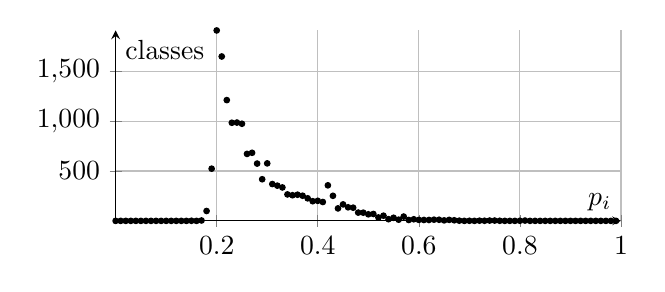
\begin{tikzpicture}\begin{axis}[width=8cm,height=4cm,axis lines=middle, xlabel={$p_i$}, ylabel={classes},xmin=0, xmax=1, ymin=0, ymax=1908,grid=major]\addplot [only marks, mark size=1pt] table {
0.0 0
0.01 0
0.02 0
0.03 0
0.04 0
0.05 0
0.06 0
0.07 0
0.08 0
0.09 0
0.1 0
0.11 0
0.12 0
0.13 0
0.14 0
0.15 1
0.16 0
0.17 4
0.18 99
0.19 523
0.2 1908
0.21 1647
0.22 1210
0.23 983
0.24 985
0.25 973
0.26 671
0.27 682
0.28 574
0.29 417
0.3 576
0.31 369
0.32 353
0.33 335
0.34 265
0.35 257
0.36 262
0.37 252
0.38 226
0.39 197
0.4 201
0.41 189
0.42 356
0.43 251
0.44 125
0.45 165
0.46 136
0.47 132
0.48 83
0.49 82
0.5 66
0.51 69
0.52 34
0.53 52
0.54 17
0.55 31
0.56 12
0.57 43
0.58 9
0.59 16
0.6 10
0.61 9
0.62 9
0.63 12
0.64 11
0.65 5
0.66 10
0.67 6
0.68 2
0.69 0
0.7 1
0.71 0
0.72 2
0.73 1
0.74 3
0.75 3
0.76 1
0.77 0
0.78 0
0.79 0
0.8 1
0.81 3
0.82 0
0.83 0
0.84 0
0.85 0
0.86 0
0.87 0
0.88 0
0.89 0
0.9 0
0.91 0
0.92 0
0.93 0
0.94 0
0.95 0
0.96 0
0.97 0
0.98 0
0.99 0
};\end{axis}\end{tikzpicture}

  \caption{Distribution of cohesion probabilities}
  \label{fig:3}
\end{figure}

It is also visually obvious that the larger the class, the lower
its cohesion. Even though it was intuitively understandable, the empirical
analysis of a large number of Java classes proved that the size of a class
negatively affects its cohesion and maintainability. It seems to be a more
complex task to keep a class highly cohesive when its size grows.

%%%%%%%%%%%%%%%%%%%%%%%%%%%%%%%%%%%%%%%%%%%%%%%%%%%%%%%%%%%%%%%%%%%%%%%%%%%%%%%%%%%%%%%%%%%%%%%%%%%%%%%%%%%%%%%%%%%%%%%
%%%%%%%%%%%%%%%%%%%%%%%%%%%%%%%%%%%%%%%%%%%%%%%%%%%%%%%%%%%%%%%%%%%%%%%%%%%%%%%%%%%%%%%%%%%%%%%%%%%%%%%%%%%%%%%%%%%%%%%
%%%%%%%%%%%%%%%%%%%%%%%%%%%%%%%%%%%%%%%%%%%%%%%%%%%%%%%%%%%%%%%%%%%%%%%%%%%%%%%%%%%%%%%%%%%%%%%%%%%%%%%%%%%%%%%%%%%%%%%
\section{Discussion}

Here is a practical comparison example of two Java libraries for sending emails.
The first one is \code{commons-email} (version 1.5) by Apache
with a large mutable class \code{SimpleEmail} at the core.%
\footnote{\url{http://commons.apache.org/proper/commons-email/}}
The second one is \code{jcabi-email} (version 1.10) with a set of immutable classes.%
\footnote{\url{http://www.jcabi.com}}

Here is how Java source code may look if it sends an email using \code{commons-email}:

\begin{minted}{text}
Email email = new SimpleEmail();
email.setHostName("smtp.googlemail.com");
email.setSmtpPort(465);
email.setAuthenticator(new DefaultAuthenticator("user", "pwd"));
email.setFrom("yegor256@gmail.com", "Yegor Bugayenko");
email.addTo("friend@jcabi.com");
email.setSubject("How are you?");
email.setMsg("Hi, how are you?");
email.send();
\end{minted}

Here is how the same email sending scenario would be
implemented with \code{jcabi-email}:

\begin{minted}{text}
Postman postman = new Postman.Default(
  new SMTP("smtp.googlemail.com", 465, "user", "pwd")
);
Envelope envelope = new Envelope.MIME(
  new Array<Stamp>(
    new StSender("Yegor Bugayenko <yegor256@gmail.com>"),
    new StRecipient("friend@jcabi.com"),
    new StSubject("How are you?")
  ),
  new Array<Enclosure>(
    new EnPlain("Hi, how are you?")
  )
);
postman.send(envelope);
\end{minted}

In the first example, it is a monster \code{SimpleEmail} class that can do many things, including
sending MIME messages via SMTP, creating the message, configuring
its parameters, adding MIME parts to it, and so on. There are 33 private properties, over
a hundred methods, and about two thousand lines of code.

In the second example, there are seven objects instantiated via seven \code{new} calls.
\code{Postman} is responsible for packaging a MIME message; \code{SMTP} is
responsible for sending it via SMTP; stamps (\code{StSender}, \code{StRecipient},
and \code{StSubject}) are responsible for configuring the MIME message before
delivery; and enclosure \code{EnPlain} is responsible for creating a MIME part
for the message, which is going to be sent. These seven objects are constructed,
encapsulated one into another, and then the postman is asked to \code{send()}
the envelope over the wire.

From a user perspective, there is almost nothing wrong. \code{SimpleEmail} is a powerful
class with multiple controls; just hit the right one and the job
gets done. However, from a developer perspective, the \code{SimpleEmail} class is
very difficult to maintain, mostly because the class is very big.
Multiple getters and setters, which are the control points of the class, modify
object attributes, configuring its behavior. When new functionality is
required, a developer has to add new attributes to the class and a new
pair of setters and getters. Of course, such a modification decreases the
cohesion of the class since there is very little or no interconnection
between newly added attributes and previously existing ones. Every new method
added to such a big class turns into an isolated island of functionality
with its own set of attributes.

Cohesion metrics are designed to spot such isolated parts inside classes and
raise red flags. A class can't be cohesive it if consists of a few logical
blocks without a strong interconnection between them.

The immutability of a class makes it difficult to make a class larger
without spending a substantial amount of effort on refactoring.
If the \code{SimpleEmail} class was immutable
in the beginning, it wouldn't be possible to add so many methods into it
and encapsulate so many properties because an immutable object only accepts a state
through its constructors. It's difficult to imagine a 33-argument constructor.
When a class is immutable from the start, its developers are forced
to keep it cohesive and small because they can't encapsulate
too much or modify what's encapsulated. Just two or three
arguments of a constructor and the reasonable limit is reached; everything
on top of that will look strange and clumsy.

The immutable design of \code{jcabi-email} implements the exact same
email sending functionality, but employs seven classes for that, instead
of one. Of course, the cohesiveness of each of them is much higher than
the one of \code{SimpleEmail}. The length of each of them is below 300
lines of code, which by itself is a perfect indicator of high readability
and maintainability.

Moreover, to extend the functionality of the library, existing classes
don't need to be modified. Each new feature must be added through
the creation of new classes and implementing existing interfaces.


%%%%%%%%%%%%%%%%%%%%%%%%%%%%%%%%%%%%%%%%%%%%%%%%%%%%%%%%%%%%%%%%%%%%%%%%%%%%%%%%%%%%%%%%%%%%%%%%%%%%%%%%%%%%%%%%%%%%%%%
%%%%%%%%%%%%%%%%%%%%%%%%%%%%%%%%%%%%%%%%%%%%%%%%%%%%%%%%%%%%%%%%%%%%%%%%%%%%%%%%%%%%%%%%%%%%%%%%%%%%%%%%%%%%%%%%%%%%%%%
%%%%%%%%%%%%%%%%%%%%%%%%%%%%%%%%%%%%%%%%%%%%%%%%%%%%%%%%%%%%%%%%%%%%%%%%%%%%%%%%%%%%%%%%%%%%%%%%%%%%%%%%%%%%%%%%%%%%%%%
\section{Conclusion}

It was demonstrated by the empirical analysis of almost a thousand
Java open source libraries and 40 thousand Java classes
that immutable classes are smaller and more cohesive, which
makes them more maintainable. Hence, it is advised to make classes
immutable to increase the overall quality of the software.

Many thanks to the contributors who
helped design and implement jPeek open-source Java software, including,
but not limited to (in alphabetic order):
Mihai Andronache,
George Aristy,
Sergey Kapralov,
Sergey Karazhenets,
Paulo Lobo,
Vladimir Motsak,
Alonso A. Ortega,
Rok Pov\v{s}i\v{c},
Vseslav Sekorin,
and
Mehmet Yildirim.

\bibliographystyle{ACM-Reference-Format}
\bibliography{main}

\end{document}
